\hypertarget{gaugefieldreader_8cpp}{}\section{gaugefieldreader.\+cpp File Reference}
\label{gaugefieldreader_8cpp}\index{gaugefieldreader.\+cpp@{gaugefieldreader.\+cpp}}


Contains the implementation of the \hyperlink{classGaugeFieldReader}{Gauge\+Field\+Reader} class methods.  


{\ttfamily \#include \char`\"{}Utils/clusterspecifier.\+h\char`\"{}}\\*
{\ttfamily \#include $<$mpi/mpi.\+h$>$}\\*
{\ttfamily \#include $<$vector$>$}\\*
{\ttfamily \#include $<$cstdio$>$}\\*
{\ttfamily \#include $<$string$>$}\\*
{\ttfamily \#include $<$ctime$>$}\\*
{\ttfamily \#include $<$cmath$>$}\\*
{\ttfamily \#include $<$random$>$}\\*
{\ttfamily \#include \char`\"{}lqcd.\+h\char`\"{}}\\*
Include dependency graph for gaugefieldreader.\+cpp\+:\nopagebreak
\begin{figure}[H]
\begin{center}
\leavevmode
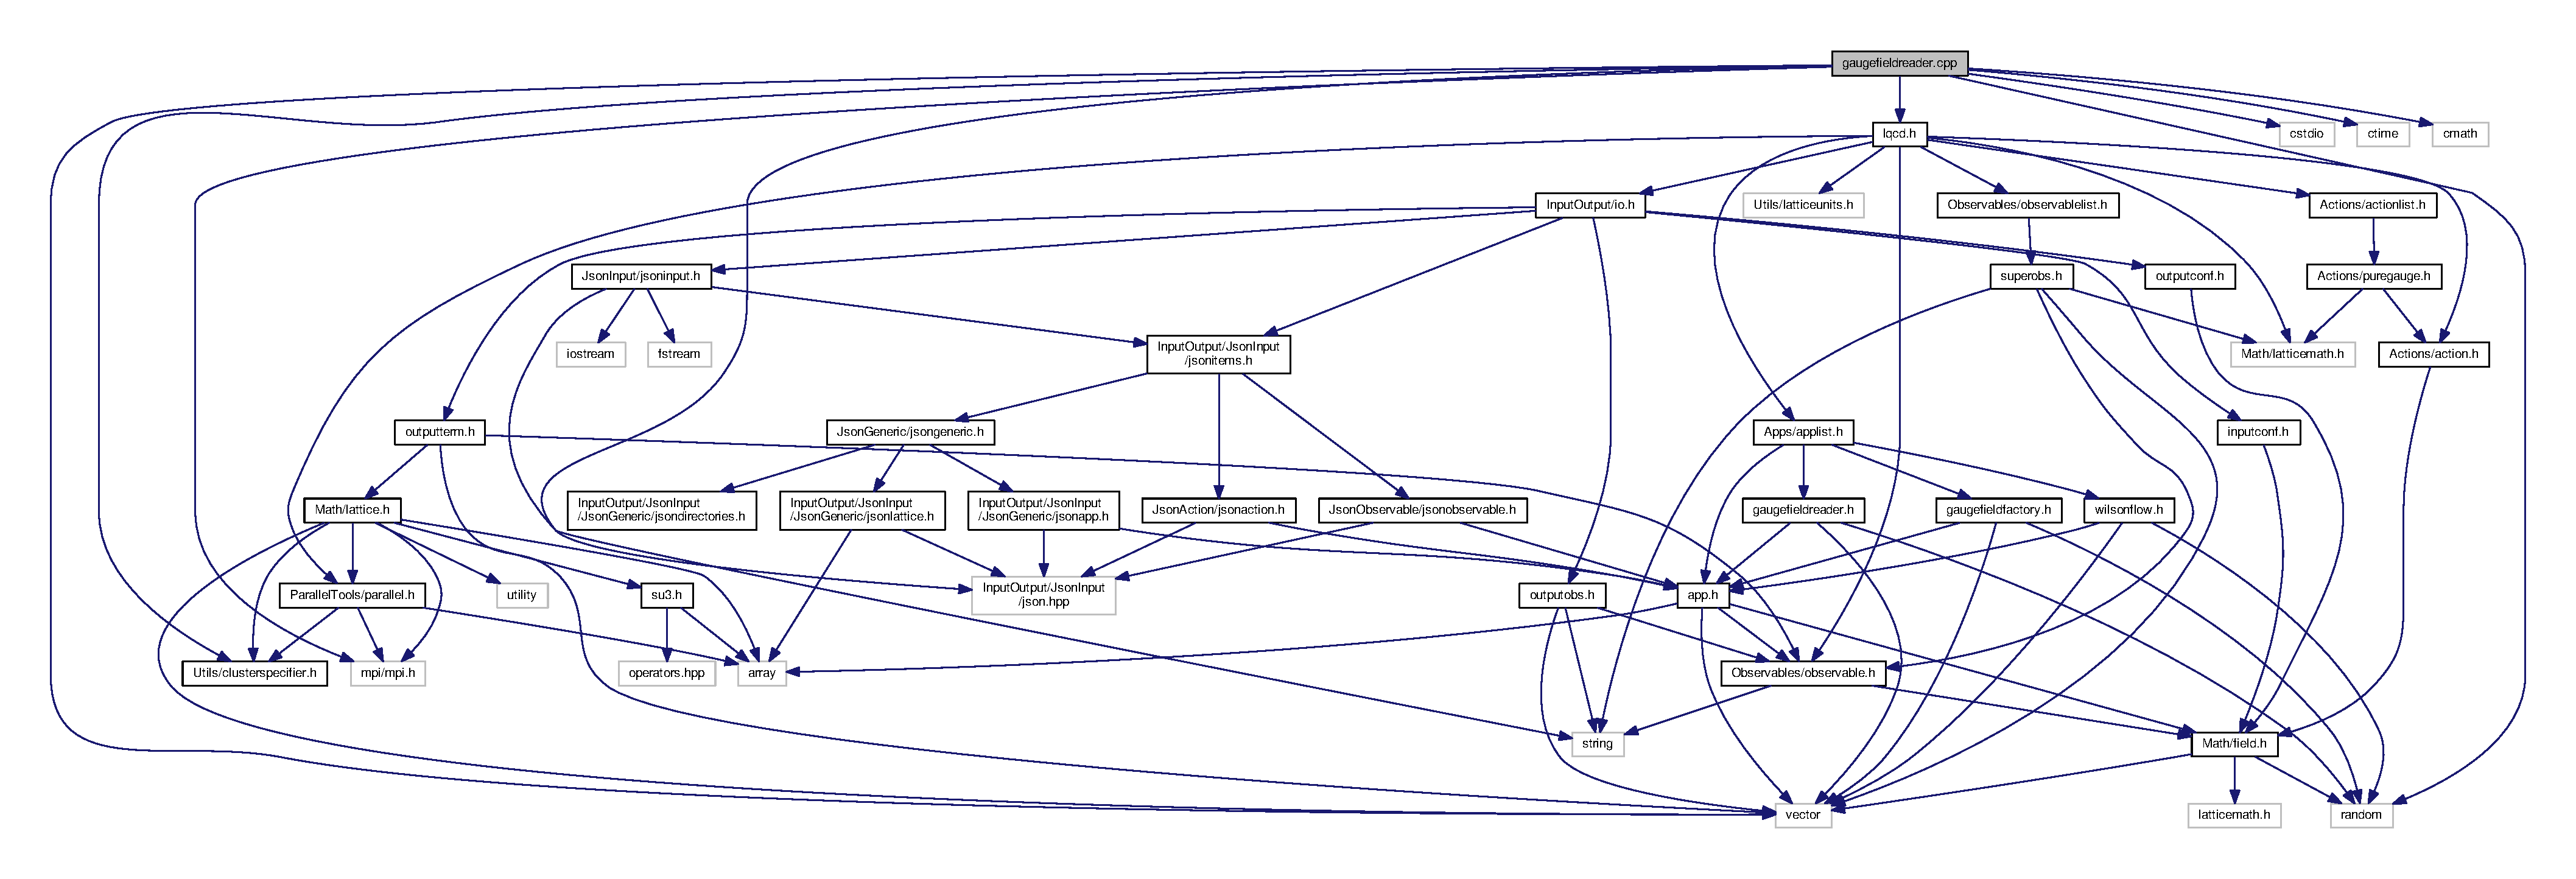
\includegraphics[width=350pt]{d1/d00/gaugefieldreader_8cpp__incl}
\end{center}
\end{figure}


\subsection{Detailed Description}
Contains the implementation of the \hyperlink{classGaugeFieldReader}{Gauge\+Field\+Reader} class methods. 

\begin{DoxyAuthor}{Author}
Giovanni Pederiva 
\end{DoxyAuthor}
\begin{DoxyVersion}{Version}
1.\+0 
\end{DoxyVersion}
\begin{DoxyDate}{Date}
2017-\/2018 
\end{DoxyDate}
\begin{DoxyCopyright}{Copyright}
M\+IT License. 
\end{DoxyCopyright}
